\documentclass[conference]{IEEEtran}
% \IEEEoverridecommandlockouts
% The preceding line is only needed to identify funding in the first footnote. If that is unneeded, please comment it out.
% \usepackage{cite}
\usepackage{amsmath,amssymb,amsfonts}
\usepackage{algorithmic}
\usepackage{graphicx}
\usepackage{textcomp}
\usepackage{hyperref}
\usepackage{flushend}

\hypersetup{
    colorlinks=true,
}
\usepackage{xcolor}
% \usepackage[backend=biber,style=numerical,sorting=ynt]{biblatex}
\usepackage[backend=biber,style=numeric,sortcites,sorting=nty,natbib,hyperref]{biblatex}


\addbibresource{sample.bib} %Imports bibliography file

\def\BibTeX{{\rm B\kern-.05em{\sc i\kern-.025em b}\kern-.08em
    T\kern-.1667em\lower.7ex\hbox{E}\kern-.125emX}}
\begin{document}

\title{Runtime Tradeoff in Traffic Monitoring Embedded Systems\\
    % {\footnotesize \textsuperscript{*}Note: Sub-titles are not captured in Xplore and
    % should not be used}
    % \thanks{Identify applicable funding agency here. If none, dont  delete this.}
}


\author{
    \IEEEauthorblockN{Pranjal Aggarwal}
    \IEEEauthorblockA{\textit{2$^{nd}$ Year UG Student} \\
        \textit{Dept. of Computer Science and Engineering} \\
        \textit{Indian Institute of Technology, Delhi}\\
        New Delhi, India. \\
        cs5190443@iitd.ac.in}
    \and
    \IEEEauthorblockN{Harsh Agrawal}
    \IEEEauthorblockA{\textit{2$^{nd}$ Year UG Student} \\
        \textit{Dept. of Computer Science and Engineering} \\
        \textit{Indian Institute of Technology, Delhi}\\
        New Delhi, India. \\
        cs1190431@iitd.ac.in}
}



\maketitle
\thispagestyle{plain}
\pagestyle{plain}

\begin{abstract}
    In this report, we have analyzed the effect of various computational parameters, and their effect on
    accuracy on the computer vision based traffic monitoring systems.
\end{abstract}

% \begin{IEEEkeywords}
% component, formatting, style, styling, insert
% \end{IEEEkeywords}

\section{Introduction}
The recent development of Smart Cities has resulted in an increase in systems capable of monitoring
road traffic for environmental analysis and better traffic management. This requires solutions such as embedded systems,
performing live inference from camera feed of CCTV cameras, deployed across many highways, expressways, and road junctions in the city.
However, these embedded systems are limited on computational capacity and may not have a significant energy source (primarily relying on solar energy).
Also, based on the time of day and day of the year, the varying temperatures add a restriction on how much computational power they can spend without getting overheated.
In this report, we investigate the various computational parameters that can be tweaked, such that the computational load on embedded systems decreases while maintaining
the performance as much as possible. Since we do not have Ground Truth Data,  we create a baseline model, which practically takes the most significant time but is assumed to be the most accurate.
All other models are evaluated against this baseline model. We use Mean Squared Error to analyze the trade-off between the time taken and utility of the model.
The following sections are divided as follows:
In the next section, we will discuss the basic algorithm of the model developed by us to calculate traffic density. This is followed by a section on the metrics used and our
approach to study the effect of runtime and utility. Further in the section, we develop a framework that can assist these systems to make dynamic decisions based on ambient conditions.
In Section 5, we discuss the Trade-Off Analysis, after which we conclude in Section 6.


% \begin{figure}[htbp]
% \centerline{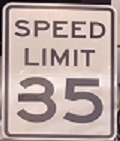
\includegraphics{tesla_speed.png}}
% \caption{By placing a 2 inch black tape on top of sign board researchers tricked a tesla car into speeding to 85mph}
% \label{tesla_speed}
% \end{figure}


\section{Algorithm}

We run our algorithm on real footage from a CCTV camera installed at Lajpatnagar junction in New Delhi. \cite{b1}
The camera has a wide range and also doesn't gives a bird's eye view. To solve this, we initially crop each of the frames and correct its perspective to get a bird's eye view.
For perspective transform, we use OpenCV's \verb|findHomography| and \verb|warpPerspective| algorithm. \cite{b2}
The region to be cropped for a junction is fixed (given the camera orientation) and is taken from the user or is hardcoded.
Then, the background from this image is removed using the \verb|MOG2| algorithm. The algorithm can be trained on an empty photo of the road or using the first few input video frames.
The image is then processed through a series of dilations and erosions, after which we perform binary thresholding. This creates a map of all the vehicles, and helps in calculation of {\bfseries{queue traffic density}}.
We have deployed two models for \textbf{dynamic density} calculation; one uses Gunner Farneback's algorithm \cite{b4} for solving optical flow equations, while the other is Lucas-Kanade's optical flow algorithm. \cite{b5}
While the former is slower, it yields better results. These algorithms can be switched depending on the computational power available.

\section{Metrics}

Utility error for a given set of test parameters is defined as the mean squared error of densities with respect to the baseline parameters. The error sum is averaged over the entire length of the video. The definition implies greater the error, lesser is the utility and vice versa.
The runtime for a set of parameters is defined as the execution time for processing the video file with the test parameter as input. To ensure results are not varied due to other computer tasks,
program runs are made on Linux Environment without explicitly running any additional software. For each set of parameters, three runs are performed, and their average is taken to further ensure that external factors do not perturb results.
\section{Methods}

To study the effect of runtime and utility we consider five optimizations:
\begin{itemize}
    \item Frame Sub-Sampling
    \item Image Resolution Reduction
    \item Multi Threading (Spatial)
    \item Multi Threading (Temporal)
    \item Using Sparse Optical Flow
\end{itemize}

In this section effect on utility for each of these is studied independently. The metrics are varied and corresponding
utility is observed and plotted. Analysis of each of these methods is included in the following subsections itself.

\subsection{Frame Sub-Sampling}

In this method, we only take every $x^{th}$ frame of the video for processing. For the skipped frames, we interpolate the density values from previous frames. We observe that as we increase the number of frames skipped, the time decreases, however the error continuously increases [See Fig~\ref{skf_evt}].
However, we also note that runtime does not change much after skipping more than four frames possibly because loading frames from video starts having a larger relative effect.
Thus we can say for the given model, setting \verb|skip_frames| to 5, is best
when running on limited performance, as it is able to improve the runtime by a factor of $\approxeq$ 2.5.

\begin{figure}[htbp]
    \centerline{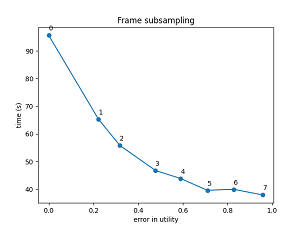
\includegraphics{plots/plot_skip_frames.png}}
    \caption{We observe, no suitable advantage is visible on skipping more than 5 frames.}
    \label{skf_evt}
\end{figure}


\subsection{Image Resolution Reduction}

In this method, we reduce the resolution of each frame by a factor. The conversion is done in realtime, and all the processing takes place on this downscaled image.
Unlike frame subsampling, we observe a linearly decreasing graph. However, the difference in error in both of these graphs is significant, with frame subsampling outperforming the current method.

\begin{figure}[htbp]
    \centerline{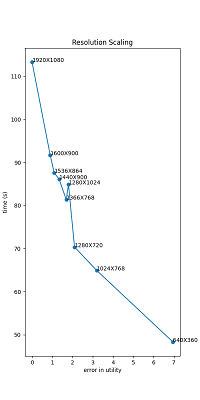
\includegraphics[scale=0.55]{plots/plot_resolution.png}}
    \caption{An almost linear increase in utility error with decrease runtime is observed}
    \label{res_evt}
\end{figure}


\subsection{Multi-Threading}
Initially, our code was single-threaded, executing statements sequentially, but many independent processes can be executed in parallel to improve the execution time.
We introduced multi-threading in our code to improve the performance by utilizing all cores of a multi-core processor. We have implemented a single producer, multiconsumer threading model using \verb|semaphores|.
A single producer reads the frame from the input video file and places it into a shared buffer. In a multi-threaded environment, several consumer threads are spawned, which wait for the
producer and start processing the frame. \verb|semaphores| are used for thread synchronization and to prevent race conditions among threads for shared memory.

\subsubsection{Spatial}
We split a frame into segments and assigned each segment to an independent thread. Splitting a frame reduces the matrix size required for each computation and lowers the
thread's average processing time. However, this method also introduces a considerable amount of errors since no thread operates on the borders.
Also, we observe that increasing threads up to 4 has some advantages; however, the runtime also starts growing. One of the reasons is that maintaining a large number of threads
has its own overhead. Moreover, since the sizes of images become small, the runtime advantage of vectorized algorithms is lost.

\begin{figure}[htbp]
    \centerline{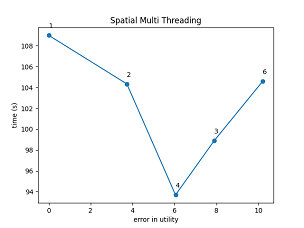
\includegraphics{plots/plot_split_frame.png}}
    \caption{We observe to get the least time, 4 threads are needed.}
    \label{smt_evt}
\end{figure}


\subsubsection{Temporal}
We split the work temporally by giving consecutive frames to different threads for processing. The analysis was parameterized by the number of threads used for processing. This method proved quite effective and practically feasible. As the number of threads was increased, the processing time decreased without any significant loss in utility.
However, there was no runtime improvements after more than four parallel threads were used. Because processors have a limit on the number of threads they can use in parallel, and OpenCV algorithms are already heavily vectorized, the saturation is reached early.

\begin{figure}[htbp]
    \centerline{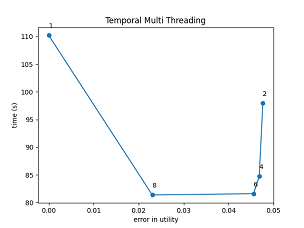
\includegraphics{plots/plot_split_video.png}}
    \caption{No sufficient advantage is seen after increasing parallel threads to more than four}
    \label{tmt_pvt}
\end{figure}

\subsection{Sparse Optical Flow}

In this method, we implement the sparse optical flow method for dynamic density calculation instead of the dense optical flow method.
We observe a significant reduction in time taken (roughly 1.8 times). However, the error observed is higher than the other methods.
This behavior is partly due to the sparse method's ability to give zero output when there is actually no movement in the road. This is in contrast to the dense optical flow method,
where there is always some noise. Sparse optical flow yields sufficiently low errors with respect to GroundTruth, and improved runtime. Hence it is an excellent method to keep the computational load in check.

\begin{figure}[htbp]
    \centerline{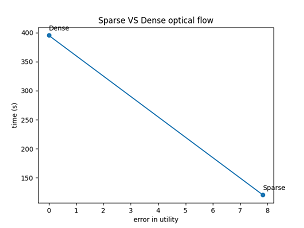
\includegraphics{plots/plot_sparse_optical.png}}
    \caption{While decrease in runtime is substantial, we observe error is substantial.}
    \label{sof_pvt}
\end{figure}

\begin{figure}[htbp]
    \centerline{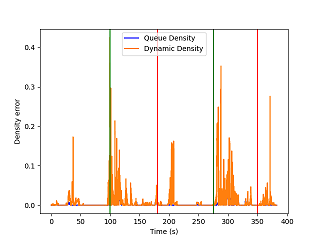
\includegraphics{plots/plot_sparse_dense.png}}
    \caption{High Error is observed at points with high dynamic density}
    \label{sparse_frame_error}
\end{figure}

\subsection{Dynamic Tuning}

For embedded systems deployed in production, they must adapt to the environmental conditions. Also, traffic monitoring systems should adjust to the traffic conditions,
i.e, when traffic is low, these embedded systems must switch to low power mode.
However, it should be noted that facilitating the same is a non-trivial problem. The reason is that different parameters do not correlate with each other in terms of error. Also, no mathematical function exists to map given error to runtime or vice-versa correctly.
To make this dynamic tuning possible, we executed the program on vast combinations of tunable parameters and created a database from the same.
Using a simple c++ function call, based on the error/time constraint, the best metric satisfying the given conditions with the best performance/least error is returned. This best metric is searched from the databse we have created. For example, in a real system, a temperature sensor can send information to tune down performance by $x\%$ and
the c++ function will return the parameters to be used for the least error.

\begin{figure}[htbp]
    \centerline{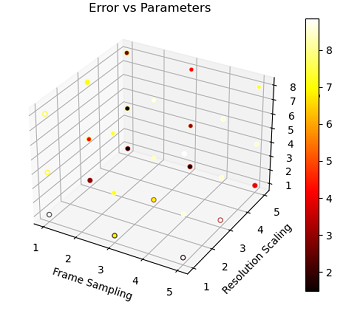
\includegraphics{plots/Error_vs_Params.png}}
    \caption{Here z-axis denotes the number of temporal threads used.}
    \label{ca_evp}
\end{figure}

\begin{figure}[htbp]
    \centerline{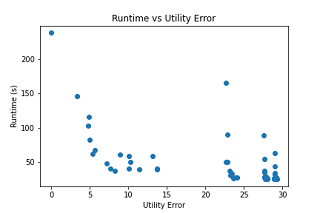
\includegraphics{plots/CompleteAnalysis_rVe.png}}
    \caption{The parameters corresponding to bottom left portion of graph are best to use when on a low computational budget}
    \label{ca_rve}
\end{figure}

\section{Trade-Off Analysis}

For the various methods, we observe that all have their own advantages. However, we note that frame subsampling can reduce the computational load significantly with the smallest decrease in error.
While temporal multi-threading reduces runtime with no significant error, it is computationally expensive due to multithreading. At the same time, multithreading's full advantage is not
observed as OpenCV algorithms are already vectorized and optimized, leaving little scope for improvements in user-created threads.
In this report, we also studied the net effect of adjusting various parameters. We observe that parameters are not additive. For example impact of sparse optical flow on lower resolution in terms of time is negligible, however, it induces greater absolute error than on high-res images.
In fact, the best compute-friendly parameters are without sparse optical flow [See Fig.~\ref{ca_rve}].
We also observe that error is maximum during transition zones when either green light turns red or vice-versa. Or in other words, the error is proportional to the queue density, however measuring error relatively, it's roughly the same for the whole video sequence.
Overall we observe choosing the right set of parameters can decrease computational time significantly (as high as 8-9 times) with minimal error.


\begin{figure}[htbp]
    \centerline{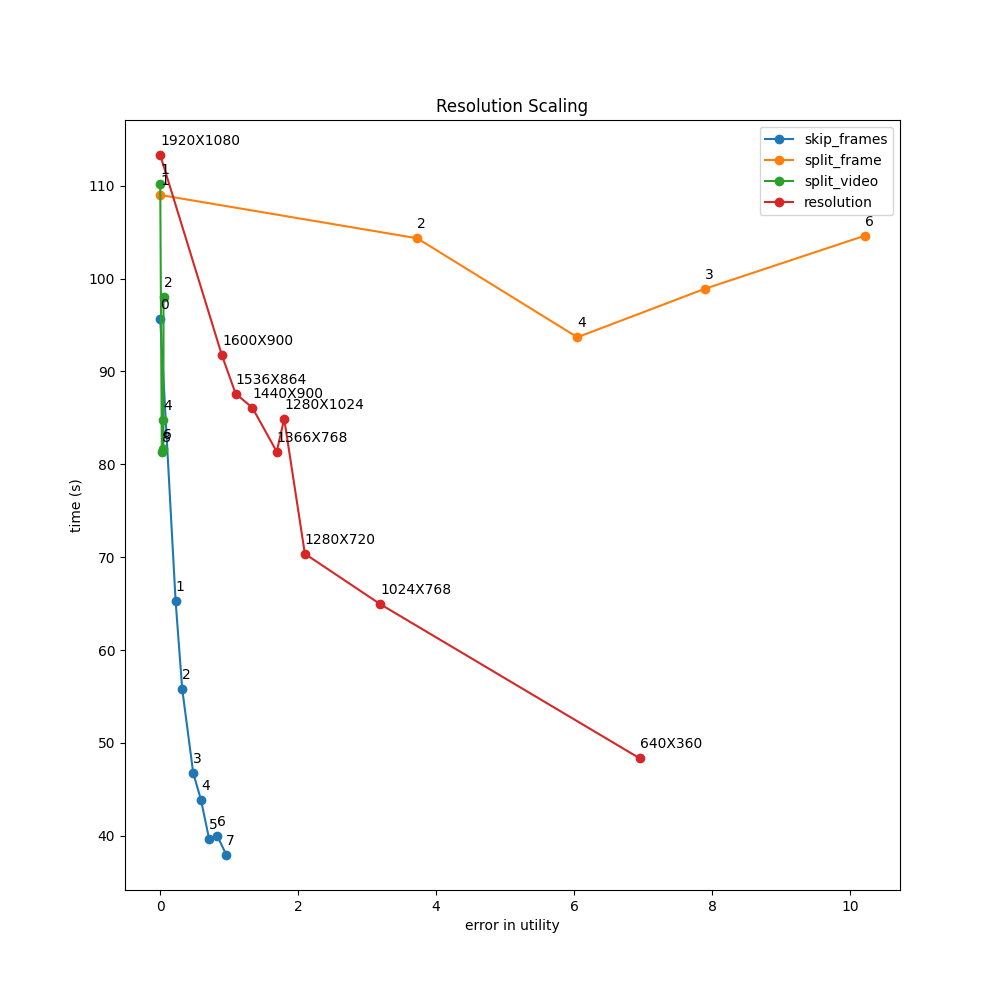
\includegraphics[scale=0.3]{plots/plot_all.png}}
    \caption{Skip Frames (blue) ensure maximum improvement in runtime without loss in much error.}
    \label{plot_all}
\end{figure}


\begin{figure}[htbp]
    \centerline{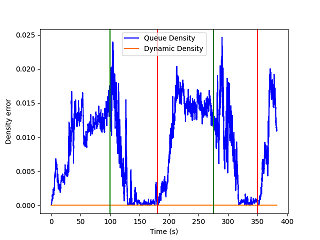
\includegraphics{plots/plot_lowres_error.png}}
    \caption{Error is high wherever traffic density is high}
    \label{low_res_err}
\end{figure}
% Graph of all methods combined(eVt) goes here

\section{Conclusion}

In this report, we have studied the effect of tuning parameters on runtime parameters for real-time computer vision based traffic monitoring system.
We see most methods are able to reduce the runtime significantly, with a minor penalty in the accuracy.
We observe that while some methods(frame subsampling) can outperform other methods in almost all cases, to improve the overall runtime, the right combination of multiple methods is needed.
However, if oa single method is used, adjusting frame subsampling to improve runtime is the best choice. Since traffic densities change at a scale of few seconds, decreasing the processing frame rate to 2 FPS will not affect the calculations much.
Overall, we conclude that naive models can be improved substantially by suitable optimizations, making it possible for real-time inference even in embedded systems.




\vspace{12pt}

\end{document}
